\subsection{Princípios da Notação Visual}\label{2-fundamentacao-notacao-visual-principios}

Historicamente, pesquisadores e projetistas de notações visuais ignoraram ou subestimaram princípios básicos da sintaxe para representar visualmente elementos de um modelo~\cite{MOODY-2009-Physics-Notation}. O desenvolvimento das notações visuais existentes em diversas áreas de conhecimento, como na engenharia de \textit{software}, foi, em sua maioria, visando atender apenas a detalhes semânticos, pouco atentando a convenções visuais.

De modo a projetar notações visuais cognitivamente eficazes, otimizando, portanto, o suporte à comunicação humana e à solução de problemas, Moody propôs um conjunto de nove princípios, chamados de Física das Notações~\cite{MOODY-2009-Physics-Notation}. Estes princípios tem como base a representação visual de constructos~\cite{MOODY-2009-Physics-Notation, POPESCU-WEGMANN-2014-Using-Physics-of-Notation-SEAM}. Constructos são modelos criados mentalmente e usados por especialistas para compreender uma parte específica de um domínio ou teoria. Construções mentais ou sínteses feitas a partir da combinação de vários elementos contribuem para a definição de um constructo. Tais construções mentais têm por objetivo a compreensão da realidade que deriva das observações e percepções individuais, resultantes de experiências (passadas ou presentes) de uma pessoa.

Os princípios da Física das Notações concentram-se nas propriedades físicas de uma notação (perceptivo) em vez de suas propriedades lógicas (semânticas). Eles foram sintetizados a partir de evidências empíricas de uma ampla variedade de domínios e baseiam-se em uma teoria explícita de como as notações visuais se comunicam. Esses princípios podem ser usados para construir novas notações visuais, bem como para avaliar, comparar e melhorar as notações visuais existentes. Cada princípio é independente dos demais, podendo ser aplicados separadamente.

\subsubsection{Princípio da Integração Cognitiva}\label{2-fundamentacao-notacao-visual-principio-integracao-cognitiva}

Notações visuais devem ter informações (representações) integradas entre diferentes modelos. Ou seja, se um elemento é representado em dois modelos distintos, este elemento deve possuir a mesma representação visual em ambos os modelos. Este princípio apenas se aplica quando múltiplos modelos são usados. Os modelos podem ser do mesmo tipo (integração homogênea) ou de tipos diferentes (integração heterogênea). Mecanismos de integração cognitiva referem-se a integrações conceituais (sumarização e momento visual) e integrações perceptivas (sinalização, orientação e mapa de navegação).

\subsubsection{Princípio do Ajuste Cognitivo}\label{2-fundamentacao-notacao-visual-principio-ajuste-cognitivo}

Notações visuais devem ter diferentes dialetos para diferenciar a comunicação entre diferentes públicos-alvos (audiência). O público-alvo pode ser composto por especialistas ou por iniciantes em um dado domínio. Diferentes dialetos visuais também podem ser necessários para diferentes objetivos (tarefas). Notações cognitivamente eficazes para uma audiência iniciante podem não ser cognitivamente eficazes para uma audiência de especialistas e vice-versa. O princípio do ajuste cognitivo afirma, portanto, que variações de uma mesma notação visual são necessárias e devem ser utilizadas conforme a audiência e os diferentes objetivos que pretende-se atingir com o uso de um dado modelo.

\subsubsection{Princípio da Diferenciação Perceptiva}\label{2-fundamentacao-notacao-visual-principio-diferenciacao-perceptiva}

Notações visuais devem ser claramente distinguíveis umas das outras. Esta distinção pode ser obtida aumentando as diferenças visuais entre as notações. Características como tamanho, forma e cor (expressividade visual) contribuem efetivamente na distinção de elementos visuais. Neste sentido, diferentes constructos semânticos devem ser facilmente identificados de acordo com suas diferentes (distintas) notações visuais. Informações textuais (codificação dupla) também podem ser utilizadas a fim de facilitar esta distinção.

\subsubsection{Princípio da Complexidade Gerenciável}\label{2-fundamentacao-notacao-visual-principio-complexidade-gerenciavel}

Modelos podem se tornar bastante complexos, dependendo diretamente da complexidade dos domínios em que eles estão sendo utilizados e do conhecimento que pretende ser representado~\cite{MOODY-2009-Physics-Notation}. Esta complexidade diagramática pode também ser medida pela quantidade de elementos visuais de um modelo. Quanto mais detalhada e granular a representação visual de um conhecimento, maior é a complexidade de um modelo. Neste sentido, notações visuais devem incluir mecanismos explícitos para lidar com modelos complexos, como, por exemplo, por meio da divisão destes em sub-modelos.

A complexidade pode também ser tratada por meio da modularização de um modelo complexo. A modularização envolve tanto a criação de modelos mais genéricos (com menos detalhes), de modo a obter uma visão mais abstrata do modelo, quanto a criação de modelos mais específicos (com mais detalhes), de modo a obter uma visão mais concreta e realista do modelo em desenvolvimento.

%A divisão de um modelo, realizada por meio da modularização e da divisão de uma estrutura hierárquica, possibilita a criação, portanto, de modelos mais genéricos (com menos detalhes) e de modelos mais específicos (com mais detalhes). Modularização refere-se a ter modelos mais genéricos, estes a fim de obter-se uma visão generalizada (simplista) do modelo, e modelos mais específicos, contendo um maior nível de granularidade e detalhes, a fim de obter-se uma visão especializada em um dado contexto do modelo que pretende-se representar visualmente.

\subsubsection{Princípio da Clareza Semiótica}\label{2-fundamentacao-notacao-visual-principio-clareza-semiotica}

O princípio da clareza semiótica relata que um constructo semântico (conceito) deve ser representado por exatamente um elemento gráfico (visual) e vice-versa~\cite{MOODY-2009-Physics-Notation}. Ou seja, deve haver uma relação 1:1 (um-para-um) entre constructos semânticos e notações visuais.

Há quatro formas de violação deste princípio, chamadas de anomalias da clareza semiótica: i) redundância de símbolos, i.e., um constructo semântico é representado por várias notações visuais; ii) sobrecarga de símbolos, i.e., uma notação visual representa mais de um constructo semântico; iii) excesso de símbolos, i.e., a notação visual é criada e não representa qualquer constructo semântico; e, por fim, iv) carência de símbolos, i.e., não há nenhuma notação visual prevista para um certo constructo semântico.

A \figurename~\ref{elementofig:anomalias-clareza-semiotica} resume as quatro anomalias da clareza semiótica. Os elementos \texttt{C\textsubscript{i}}, à esquerda, representam constructos semânticos, enquanto que os elementos \texttt{S\textsubscript{i}}, à direita, representam símbolos.

%O elemento \texttt{C\textsubscript{1}} não possui uma representação visual. Portanto, \texttt{C\textsubscript{1}} caracteriza-se pela anomalia de carência de elementos. O elemento \texttt{C\textsubscript{2}} possui duas representações visuais: \texttt{S\textsubscript{1}} e \texttt{S\textsubscript{2}}. Portanto, \texttt{C\textsubscript{2}} caracteriza-se pela anomalia de redundância de elementos. \texttt{C\textsubscript{3}} e \texttt{C\textsubscript{4}} compartilham da mesma representação visual: \texttt{S\textsubscript{3}}. Portanto, \texttt{C\textsubscript{3}} e \texttt{C\textsubscript{4}} caracterizam-se pela anomalia de sobrecarga de símbolos. Finalmente, \texttt{S\textsubscript{4}} é uma representação visual que não possui um constructo semântico relacionado. Portanto, \texttt{S\textsubscript{4}} caracteriza-se pela anomalia de excesso de símbolos.

\begin{figure}[h]
    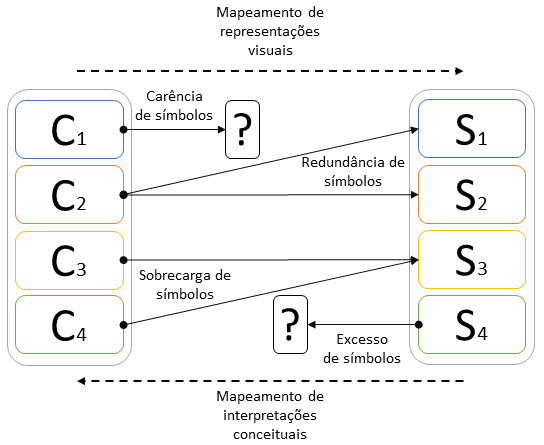
\includegraphics[scale=0.8]{2-fundamentacao-teorica/imagens/clareza-semiotica.png}
    \centering
    \caption[Anomalias do princípio da clareza semiótica.]{\textbf{Anomalias do princípio da clareza semiótica.} Adaptado de~\cite{MOODY-2009-Physics-Notation}}
    \label{elementofig:anomalias-clareza-semiotica}
\end{figure}

\subsubsection{Princípio da Expressividade Visual}\label{2-fundamentacao-notacao-visual-principio-expressividade-visal}

Notações visuais podem fazer uso de sete diferente variáveis visuais para melhorar a expressividade de uma notação visual: posição, tamanho, brilho, textura, cor, orientação e forma. A expressividade visual é determinada pelo número de variáveis visuais usadas em uma notação e a extensão em que elas são utilizadas. Porém, no contexto do nosso trabalho, as variáveis cor, tamanho, forma e posição são consideradas mais relevantes.

A cor é uma das mais importantes variáveis visuais, uma vez que o contraste de cor é interpretado mais rapidamente do que as diferenças entre outras variáveis. Porém, cores devem ser usadas com cuidado e apenas em conjunto (de forma redundante) com outras variáveis, dado que suas diferenças desaparecem quando modelos são impressos em escala de cinza ou então quando os modelos são utilizados por pessoas daltônicas.

Elementos visuais também podem ser diferenciados pelo uso de diferentes formas e tamanhos. Por exemplo, retângulos podem ser utilizados para representar atividades enquanto losangos podem ser utilizados para representar decisões na BPMN~\cite{OMG-2011-BPMN}. Em um modelo de nuvem de palavras~\cite{HEIMER-LOHMANN-LANGE-ERTL-2014-WORD-CLOUD}, o tamanho de uma dada palavra-chave é proporcional à relevância desta no modelo. Quanto mais revelante, maior é a palavra em relação às demais.

%Para diferentes tamanhos, como exemplo, podemos citar elementos mais importantes (mais relevantes) podem ter tamanhos maiores em relação à elementos menos importantes em um modelo, como é o exemplo de palavras-chave mais relevantes um dado contexto sendo representadas com tamanhos maiores em um modelo de nuvem de palavras~\cite{HEIMER-LOHMANN-LANGE-ERTL-2014-WORD-CLOUD}.

Elementos visuais podem ser diferenciados conforme o seu posicionamento, ou seja, conforme a sua posição no eixo X (horizontal) e no eixo Y (vertical). Por exemplo, em um organograma empresarial, profissionais líderes podem ser apresentados verticalmente (eixo Y) acima de seu time, bem como profissionais com o mesmo cargo podem ser apresentados no mesmo nível vertical (eixo Y), porém espaçados (distribuídos) horizontalmente (eixo X).

Diferentes brilhos e texturas também podem contribuir para uma maior expressividade visual. O brilho pode alterar a tonalidade de uma representação visual e muitas vezes é utilizado em conjunto com as cores a fim de se obter uma maior diferenciação entre elementos de um modelo. Por fim, orientações de notações visuais, como diferentes ângulos (rotações) utilizados para um mesmo elemento visual, podem contribuir para representar diferentes conceitos semânticos em um dado modelo.

\subsubsection{Princípio da Economia Gráfica}\label{2-fundamentacao-notacao-visual-principio-economia-grafica}

Notações visuais devem ser utilizadas com parcimônia, ou seja, o número de elementos gráficos deve ser limitado e de fácil gerenciamento. Um grande número de convenções aumenta a complexidade de um modelo, dificultando o seu entendimento.

A fim de satisfazer o princípio da economia gráfica, três abordagens podem ser utilizadas. A primeira abordagem refere-se à remoção de constructos semânticos, ou seja, reduz-se a quantidade de constructos semânticos e, consequentemente, de representações visuais relacionadas. Esta redução deve ser realizada com cuidado a fim de que o princípio clareza semiótica não venha a ser violado. A segunda abordagem refere-se à simples eliminação de representações visuais. Contudo, esta abordagem é mais arriscada, visto que a anomalia carência de símbolos, da clareza semiótica, pode ser mais facilmente introduzida. Por fim, a terceira abordagem refere-se ao aumento da expressividade visual. Esta abordagem pressupõe que com o aumento de características (atributos) visuais de um dado elemento, enriquecendo, portanto, a sua expressividade visual, este elemento pode ser tornar suficientemente claro para substituir simultaneamente dois ou mais elementos em um dado modelo.

\subsubsection{Princípio da Codificação Dupla}\label{2-fundamentacao-notacao-visual-principio-codificacao-dupla}

Textos contribuem para a compreensão de um modelo quando usados em conjunto com representações gráficas. Assim, notações visuais devem utilizar tanto elementos gráficos quanto elementos textuais. Uma representação textual não deve substituir uma representação gráfica, mas sim complementá-la. O uso de elementos textuais com elementos gráficos contribui para uma transmissão de informação mais efetiva do que quando usados de forma separada. Entretanto, é importante que as representações gráficas sejam distinguíveis com base nas ilustrações. Elementos como rótulos (\textit{labels}) devem ser utilizados apenas para distinguir instâncias de um mesma representação gráfica, mas não entre tipos (elementos) diferentes.

\subsubsection{Princípio da Transparência Semântica}\label{2-fundamentacao-notacao-visual-principio-transparencia-semantica}

Notações visuais devem utilizar elementos gráficos cuja aparência sugerem o significado de seus constructos semânticos. Transparência semântica avalia a facilidade com a qual uma representação visual é relacionada ao seu real significado (constructo).

A transparência semântica de um elemento pode ser classificada em: semanticamente imediata, semanticamente opaca ou semanticamente perversa. Um elemento é semanticamente imediato se um leitor iniciante é capaz de inferir o seu significado por si só a partir da sua aparência. Por exemplo, um boneco para representar uma pessoa. Um elemento é semanticamente opaco (ou convencional) se existe uma relação puramente arbitrária entre a sua aparência e seu significado. Por exemplo, um retângulo para representar uma entidade em um diagrama entidade relacionamento (DER). Finalmente, um elemento é semanticamente perverso (ou um falso mnemônico), se um leitor iniciante é susceptível a inferir um significado diferente ou até mesmo oposto ao significado do elemento. Por exemplo, uma classe pode ser interpretada como uma interface em um diagrama de classes da UML.

Uma abordagem eficaz de se modelar elementos com transparência semântica é por meio de ícones. Ícones facilitam o reconhecimento de constructos semânticos. Adicionalmente, ícones melhoram a compreensão da notação principalmente para os usuários iniciantes. Notações visuais semanticamente transparentes também reduzem a carga cognitiva, visto que elas têm mnemônicos embutidos e o seu significado pode ser percebido diretamente ou facilmente aprendido.

A \figurename~\ref{fig:transparencia-semantica} ilustra as medidas da transparência semântica. Quanto mais à direita (sinal positivo), mais um elemento visual é semanticamente imediato. Quanto à esquerda (sinal negativo), mais um elemento visual é semanticamente perverso. No centro do eixo, entre semanticamente imediato e semanticamente perverso, um elemento pode ser considerado semanticamente opaco (neutro).

\begin{figure}[h]
    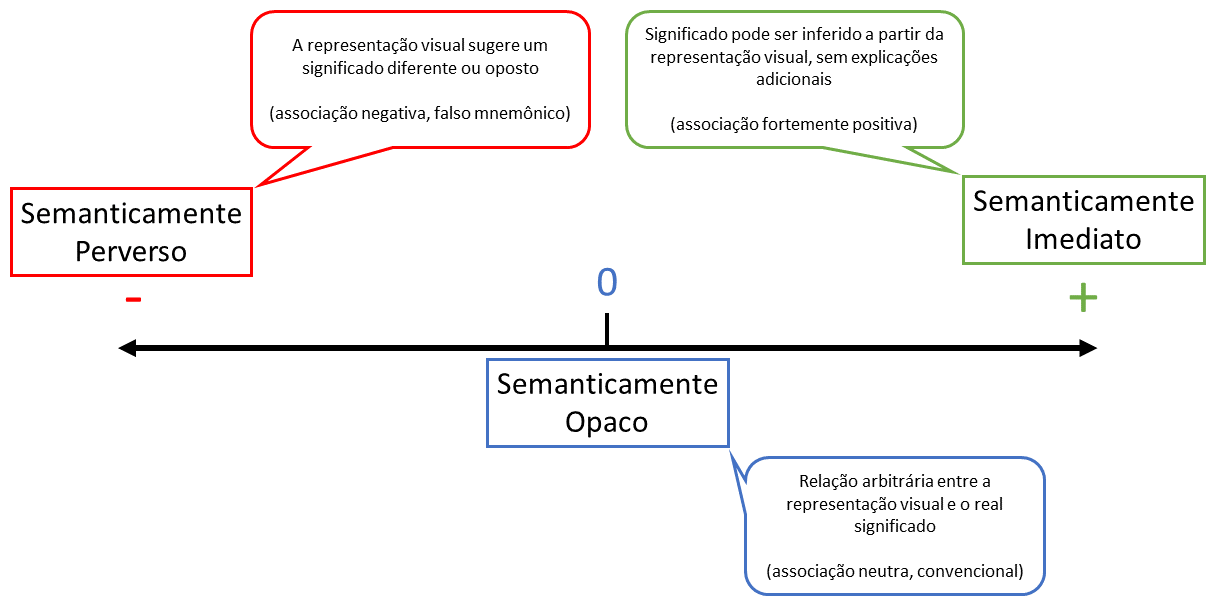
\includegraphics[scale=0.48]{2-fundamentacao-teorica/imagens/transparencia-semantica.png}
    \centering
    \caption[Princípio da transparência semântica.]{\textbf{Princípio da transparência semântica.} Adaptado de~\cite{MOODY-2009-Physics-Notation}}
    \label{fig:transparencia-semantica}
\end{figure}